\documentclass{article} % There are various classes of documents, we will see a few later
\usepackage{tikz}
\title{Basic LaTeX}
\author{J Campbell}
\date{\today}
\begin{document} % This line start the document
\maketitle
Hello, world!
\begin{abstract}
This document contains some basic LaTeX code that will be useful to me in the future.
\end{abstract}
\begin{itemize}
    \item Unorderd item number 1
    \item Unorderd item number 2
\end{itemize}

\begin{enumerate}
    \item Ordered item number 1
    \item Ordered item number 2
\end{enumerate}

\begin{tabular}{|l|c|r|}
    \hline
    Name & Gender & Start Time\\
    \hline
    Angelico & Male & 1100\\
    \hline
    Leanne & Female & 0830\\
    \hline
    Lisa & Female & 0730\\
    \hline
\end{tabular}
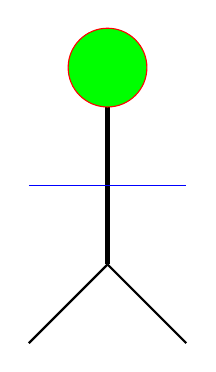
\begin{tikzpicture}
    \draw [ultra thick] (0,0) -- (0,2); % This draws a line from (0,0) to (0,2)
    \draw [thin, color=blue] (-1,1) -- (1,1); % This draws a line from (-1,1) to (1,1)
    \draw [thick] (0,0) -- (1,-1); % This draws a line from (0,0) to (1,-1)
    \draw [thick] (0,0) -- (-1,-1); % This draws a line from (0,0) to (-1,-1)
    \draw [color=red, fill=green] (0,2.5) circle(.5); % This draws a circle at (0,2.5) with radius .5
\end{tikzpicture}
\end{document}